
\newcommand{\nomedoc}{Piano Di Progetto}
\newcommand{\versione}{2.2}
\newcommand{\versioneglossario}{2.0}
\newcommand{\versionenormeprogetto}{2.0}
\newcommand{\versioneAR}{2.0}
\newcommand{\nomefile}{PianoDiProgetto-\versione.pdf}
\newcommand{\datacreazione}{11 Dicembre 2010}
\newcommand{\datamodifica}{31 Gennaio 2011}
\newcommand{\stato}{formale}
\newcommand{\uso}{esterno} 
\newcommand{\redazione}{Lovato Daniele\\& Mandolo Andrea}
\newcommand{\verifica}{Trezzi Giovanni}
\newcommand{\approvazione}{Palazzin Alberto}
\newcommand{\distribuzione}{
VT.G \\
& Prof. Vardanega Tullio\\
& Prof. Cardin Riccardo}

% FUNZIONI TIPOGRAFICHE
\newcommand{\co}{\texttt} % courier
\newcommand{\bo}{\textbf} % bold
\newcommand{\pr}{\par\medskip} % paragrafo spaziato
\newcommand{\sca}{\textsc} % small caps

\documentclass[a4paper,12pt]{report}
% 10pt,11pt,12pt
% titlepage, notitlepage -> per dare inizio o no ad una nuova pagina dopo titolo
% twoside -> per dire se fronte-retro
\usepackage[latin1]{inputenc}
% per caratteri accentati
\usepackage[italian]{babel}
% per regole sintattiche italiane
\usepackage[bookmarks=true, pdfborder={0 0 0 0}]{hyperref}
% per collegamenti ipertestuali
\usepackage{graphicx}
% per inserimento immagini

% \usepackage{enumerate}
% per personalizzare elenchi puntati

\usepackage[hmargin=2cm]{geometry} %margine 2 cm
%\geometry{options varie}

% comandi per gestire meglio header e footer
\usepackage{fancyhdr}  % header e footer
\usepackage{totpages}
\pagestyle{fancy}
\renewcommand{\headrulewidth}{0.4pt}
\renewcommand{\footrulewidth}{0.4pt}

\setlength{\headheight}{1.2cm} % NON TOCCARE
\setlength{\voffset}{-1.5cm} % NON TOCCARE
\setlength{\textheight}{666pt} % NON TOCCARE
\setlength{\footskip}{60pt}
\setlength{\parindent}{0pt} % INDENTAZIONE

\lhead{\nomedoc\  (ver. \versione)}
\chead{}
\rhead{
\includegraphics[height=1cm]{img/netmus.png}}
\lfoot{
\includegraphics[height=0.8cm]{img/logo.png}}
\cfoot{}
\rfoot{\thepage}

\usepackage{titlesec}
\titleformat{\chapter}{\normalfont\huge\bfseries}
{\thechapter}{20pt}{\Huge}

\usepackage{rotating}   % PER TABELLE E AMBIENTI RUOTATI
\usepackage{array}
\usepackage{color}
\usepackage{colortbl}  % VARIE PER GESTIRE I COLORI
\definecolor{Orange}{RGB}{255,127,0}   % ARANCIO ACCES0
\definecolor{orange}{RGB}{255,207,80}  % ARANCIO TENUE

\addtocontents{toc}{\protect\thispagestyle{fancy}}  % PER INDICI CON + PAGINE
\usepackage[font=it]{caption}    % PER RENDERE CORSIVE LE DIDASCALIE
\usepackage{eurosym}  % PER SIMBOLO EURO

% \usepackage{listings}   per codice sorgente

\author{VT.G - Valter Texas Group}

\begin{document}

\pagenumbering{Roman} % INIZIO NUMERAZIONE ARABA

\vspace*{1cm}
\begin{center}

\begin{LARGE} \sca{Federico Baron} \end{LARGE}\\
\vspace{0.5cm}
\begin{Large}
\emph{fede.baron.89@gmail.com} \end{Large}\\
\vspace*{1cm} 
\includegraphics[width=5cm]{img/logo.png}\\
\vspace{0.5cm}
\begin{Large} \emph{``Comunicazione Aumentata/Alternativa per Giovani Ospiti
della Terapia Intensiva Pediatrica''} \end{Large}\\
\vspace{3cm}
\begin{Large} \sca{\nomedoc} \end{Large}\\
\end{center}
\vspace{1cm}

% INFORMAZIONI DOCUMENTO
\begin{center}
\begin{tabular}{r|l}
\hline & \\
\bo{Nome} & \nomefile \\
\bo{Versione attuale} & \versione \\
\bo{Data creazione} & \datacreazione \\
\bo{Data ultima modifica} & \datamodifica \\
\bo{Redazione} & \redazione \\
& \\\hline
\end{tabular}
\end{center}
\newpage

\chapter*{Sommario}
\thispagestyle{fancy}
Il presente documento descrive l'organizzazione del gruppo VT.G, le
assegnazioni previste, la rotazione dei ruoli di progetto, l'impegno previsto
per ogni ruolo e per ogni membro ed il conto economico preventivo.\\
Viene inoltre presentata un'analisi dei rischi presenti durante il progetto, con
relativa strategia preventiva su di essi.

\newpage
% REGISTRO MODIFICHE
\section*{Registro delle modifiche}

\begin{longtable}{|p{0.13\textwidth}|c|p{0.2\textwidth}|p{0.46\textwidth}|}
\hline
\rowcolor{orange} \bo{Data} & \bo{Versione} & \bo{Autore} & \bo{Descrizione} \\
\hline
\endhead
\hline
\endfoot
21/02/2011 & 2.2 & Lovato Daniele & Completato consuntivo e analisi dei rischi
in fase RP-RQ.\\
\hline
10/02/2011 & 2.1 & Lovato Daniele & Sistemati errori evidenziati dalla
revisione di progetto.\\
\hline
31/01/2011 & 2.0 & Daminato Simone & Validazione per consegna RP.\\
\hline
31/01/2011 & 1.9 & Trezzi Giovanni & Verificato l'intero documento.\\
\hline
30/01/2011 & 1.8 & Caputo Cosimo & Corretti errori segnalati.\\
\hline
30/01/2011 & 1.7 & Palazzin Alberto & Verificate sezioni modificate o nuove.\\
\hline
30/01/2011 & 1.6 & Baron Federico & Completato consuntivo.\\
\hline
22/01/2011 & 1.5 & Caputo Cosimo & Corretti errori grammaticali e di
sintassi.\\
&&&Abbozzata sezione Consuntivo\\
\hline
21/01/2011 & 1.4 & Lovato Daniele & Sistemata la sezione di analisi dei
rischi con aggiunta delle strategie di gestione.\\
\hline
19/01/2011 & 1.3 & Lovato Daniele & Corretto Capitolo 3 e 4.\\
&&&Rifatta completamente la Pianificazione.\\
\hline
19/01/2011 & 1.2 & Lovato Daniele & Perfezionata Analisi dei Rischi e aggiunta
sezione Rischi nella fase RR-RP.\\
\hline
12/01/2011 & 1.1 & Mandolo Andrea & Modificato layout Registro delle
modifiche e Riferimenti.\\
\hline
19/12/2010 & 1.0 & Palazzin Alberto & Validazione per consegna RR.\\
\hline
18/12/2010 & 0.6 & Trezzi Giovanni & Verificato l'intero documento.\\
\hline
16/12/2010 & 0.5 & Mandolo Andrea & Corretti errori ortografici e sintattici.\\
\hline
13/12/2010 & 0.4 & Lovato Daniele & Corretti errori grammaticali e di
battitura.\\
&&& Aggiunti commenti ai grafici.\\
\hline
13/12/2010 & 0.3 & Mandolo Andrea & Completati contenuti dei capitoli 2-3-4.\\
\hline
12/12/2010 & 0.2 & Lovato Daniele & Aggiunta sezione analisi dei rischi.\\
\hline
11/12/2010 & 0.1 & Mandolo Andrea & Stesura prima versione del documento.\\
\end{longtable}

% INDICE
\tableofcontents

\chapter{Introduzione}
\thispagestyle{fancy} % serve perche' nelle pagine di inizio Chapter esca header e footer
\pagenumbering{arabic} % INIZIO NUMERAZIONE NORMALE
\rfoot{\thepage\ di \pageref{TotPages}}

\section{Scopo del documento}
Il piano di progetto fissa le risorse disponili nel gruppo, la suddivisione
delle attivit\`a di progetto, il calendario delle attivit\`a ed un prospetto
economico preventivo. Deve descrivere l'organizzazione delle attivit\`a di
progetto al fine di produrre risultati utili al responsabile per valutare in
maniera appropriata il progresso del lavoro.


\section{Scopo del prodotto}
Il progetto \underline{NetMus} nasce con lo scopo di realizzare un sistema
software basato su \underline{cloud} \underline{computing}, per memorizzare
informazioni di brani musicali in profili utente online.\\ Tali informazioni vengono estratte da
dispositivi musicali o di archiviazione \underline{USB} al momento della loro connessione.

\section{Glossario}
Il Glossario \`e definito con un documento a parte
(\emph{Glossario-\versioneglossario.pdf}). Tutti i termini caratterizzati da
\underline{questa sottolineatura} sono ivi definiti.\\
Verr\`a sottolineata solamente la prima occorrenza di ciascun
termine presente nel Glossario, per non compromettere la leggibilit\`a del documento.

\section{Riferimenti}

\subsection{Normativi} % oppure rif. a Norme di progetto con leggi e tutto
\begin{itemize}
  \item ISO/IEC 12207:1995 - Cicli di vita software
  \item ISO/IEC 9126:2001 - Quality Model
  \item \emph{NormeDiProgetto-\versionenormeprogetto.pdf} che regola e
  accompagna tutti i documenti ufficiali.
\end{itemize}
\newpage
\subsection{Informativi}
\begin{itemize}
  \item Capitolato d'appalto CO2-NETMUS del corso di Ingegneria del Software
  A.A. 2010/11 :\\
  \url{http://www.math.unipd.it/~tullio/IS-1/2010/Progetto/NetMus.pdf}
  \item Slide delle lezioni del corso:\\
  \url{http://www.math.unipd.it/~tullio/IS-1/2010/}
  \item Verbale intervista proponente:\\
  \co{allegato Verbale-1.0.pdf}
  \item Sistema di cloud Google App Engine:\\
  \url{http://code.google.com/intl/it/appengine/}
\end{itemize}



\chapter{Organizzazione del gruppo}
\thispagestyle{fancy}

\section{Membri del gruppo}
Il gruppo VT.G - Valter Texas Group si compone in data 26/11/2010, in previsione
del progetto didattico di Ingegneria del Software 2010/2011 inserito
all'interno del corso di laurea in Informatica dell'Universit\`a di Padova.
Dopo aver valutato e studiato i capitolati d'appalto presentati a lezione il
30/11/2010, accetta di sviluppare in data 03/12/2010 il progetto presentato nel capitolato C02 - NetMus proposto dal Prof. Cardin Riccardo.\\

Il gruppo \`e composto da 7 membri:

\begin{center}
\begin{tabular}{lcl}
\hline
\bo{Nominativo} & \bo{Matricola} & \bo{E-mail} \\
\hline
Baron Federico & 599799 & fede.baron.89@gmail.com \\
Caputo Cosimo & 524037 & caputo.cosimo85@gmail.com \\
Daminato Simone & 574545 & skyled@alice.it \\
Lovato Daniele & 578396 & danyleleorti@hotmail.com \\
Mandolo Andrea & 563175 & andrea.mandolo@gmail.com \\
Palazzin Alberto & 522095 & alberto.palazzin@gmail.com \\
Trezzi Giovanni & 487539 & giovytr@trezzi.net \\
\hline
\end{tabular}
\end{center}

\section{Ruoli di progetto}
Durante lo sviluppo del progetto saranno presenti nel gruppo i seguenti ruoli:
\begin{itemize}
  \item Responsabile
  \item Amministratore
  \item Analista
  \item Progettista
  \item Programmatore
  \item Verificatore
\end{itemize}

Tali ruoli verranno assegnati a rotazione tra i membri del gruppo, dando
cos\`\i\ la possibilit\`a a tutti di provare ogni tipo di lavoro.

\section{Attribuzione dei ruoli}
Nel capitolo 4 di Pianificazione verr\`a illustrata nel dettaglio la distribuzione dei ruoli
all'interno del gruppo, nei periodi compresi tra le varie revisioni.
In un certo periodo, garantendo assenza di conflitto d'interessi, un membro
coprir\`a pi\`u ruoli, ma sempre assicurando un'adeguata ripartizione delle ore
di lavoro individuale.\\

Per il periodo della stesura iniziale dei documenti, ciascun
componente ricopre il ruolo di analista, in modo da poter garantire una pi\`u
accurata definizione e studio dei requisiti iniziali.

\chapter{Ciclo di vita}
\thispagestyle{fancy}
Lo sviluppo del progetto NetMus seguir\`a un modello di ciclo di vita
di tipo incrementale. Una volta fissate analisi dei
requisiti e progettazione architetturale si proceder\`a con due iterazioni nelle
attivit\`a di progettazione di dettaglio e realizzazione. In questo modo si
avr\`a la possibilit\`a di correggere potenziali mancanze e migliorare il
software.\\
La prima iterazione di progettazione logica e realizzazione sar\`a la pi\`u
longeva: in essa verranno soddisfatti i requisiti obbligatori descritti nel
documento \emph{AnalisiDeiRequisiti-\versioneAR.pdf}.\\
Nella seconda iterazione invece, verranno realizzate ed integrate le parti
software che soddisfano i requisiti desiderabili ed opzionali che si \`e deciso
di implementare.\\

Questo modello, data la nostra inesperienza su progetti di tale dimensione e
sulle nuove tecnologie usate (\underline{GAE}, \underline{GWT} e
\underline{JavaFX}), ci assicura un rischio minore di fallimento: dopo la prima iterazione completa il prodotto dovrebbe
gi\`a possedere i requisiti obbligatori concordati con il committente; nella
seconda si andr\`a solamente ad aggiungere valore senza dover rivoluzionare il
lavoro gi\`a fatto.\\

Le revisioni che il gruppo VT.G dovr\`a sostenere sono:
\begin{itemize}
  \item Revisione dei requisiti (\underline{RR}): esterna;
  \item Revisione di progettazione (\underline{RP}): interna (funzione minima);
  \item Revisione di qualifica (\underline{RQ}): interna;
  \item Revisione di accettazione (\underline{RA}): esterna.
\end{itemize} \vspace{0.5cm}

`Funzione minima' alla revisione di progettazione indica che porteremo come
prodotti in ingresso la Specifica Tecnica, Piano Di Progetto v2, Piano Di
Qualifica v2 e lo stato di uscita sar\`a il prodotto specificato.\\
\\
Questa scelta \`e stata presa poich\'e riteniamo pi\`u importante avere una
valutazione esterna correttiva sulla progettazione architetturale, invece che
sulla progettazione di dettaglio.\\
\\
La Definizione Del Prodotto verr\`a sviluppata internamente durante gli
incrementi di sviluppo, cos\`\i\ come il Piano Di Progetto v3 e Piano di
Qualifica v3.


\chapter{Pianificazione}
\thispagestyle{fancy}

\section{Diagramma di Gantt}
Per facilitare la gestione oraria e il rispetto delle scadenze preposte,
forniamo un \underline{diagramma di} \underline{Gantt} che illustra in dettaglio
l'andamento delle attivit\`a del gruppo durante l'intero sviluppo del progetto.
\vspace{0.8cm}
\begin{figure}[htbp]
  \centering
  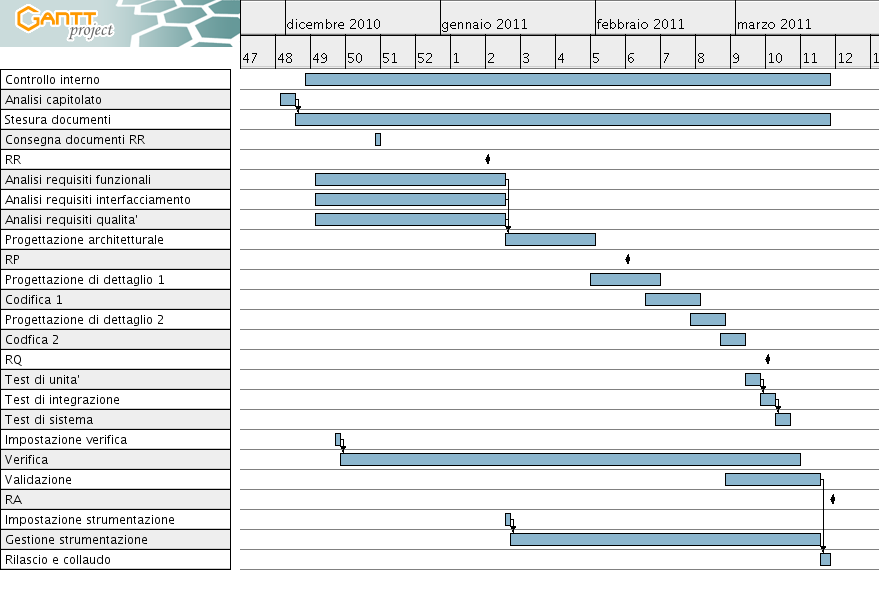
\includegraphics[width=17.2cm, angle=0]{img/PP/gantt.png}
\caption{Diagramma di Gantt}
\end{figure}
\newpage

Come si pu\`o notare dal grafico, le revisioni sono indicate come punti di 
verifica con dei piccoli rombi neri, per semplificare la visione.\\
L'attivit\`a di analisi proseguir\`a anche dopo la RR, per adattare i nostri
requisiti ad eventuali variazioni correttive emerse durante tale revisione.\\

Si pu\`o chiaramente vedere che il processo di \underline{verifica} sar\`a
presente costantemente a partire dalla stesura dei documenti, durante la progettazione e
la codifica fino ad arrivare ai test di qualifica.\\

La stesura dei documenti ricoprir\`a tutta la durata del progetto, per portare
in ingresso alle revisioni i nuovi documenti richiesti o le versioni aggiornate
di quelli precedentemente presentati.

\section{Prospetto  Economico}
Come specificato nelle richieste del progetto didattico, ciascun ruolo avr\`a un
determinato costo orario (vedi tabella sottostante) che contribuir\`a al calcolo
del costo complessivo del prodotto, che ricordiamo non dovr\`a essere
inferiore a 13.000 Euro.

\vspace{1cm}
\begin{table}[h]
\begin{center}
\begin{tabular}{|l|c|}
\hline
\rowcolor{orange}
\bo{Ruolo}  & \bo{Costo(\euro)} \\
\hline Responsabile & 30 \\ \hline
Amministratore & 20 \\ \hline
Analista & 25 \\ \hline
Progettista & 22 \\ \hline
Programmatore & 15 \\ \hline
Verificatore & 15 \\
\hline
\end{tabular}
\caption{Ruoli e costi orari}
\end{center}
\end{table}


\vspace{0.5cm}
A partire dalla consegna dei documenti per la RR, verranno tracciate le ore di
lavoro dei membri del gruppo. L'impegno totale di ciascun componente dovr\`a
essere compreso tra 85 e 105 ore, dal quale risulteranno proporzionali
ripartizioni tra carico di lavoro e responsabilit\`a.\\
\\
Di seguito riportiamo una stima dei costi per ogni periodo intermedio
tra le revisioni e il carico di lavoro previsto per ogni membro del gruppo.
Verranno inoltre illustrati il criterio ed il calendario di rotazione dei
ruoli sulle attivit\`a previste per ogni periodo.
\newpage

\subsection{RR - RP}

\vspace{0.5cm}
Periodo compreso tra la RR (10/01/2011) e la RP (07/02/2011).

\begin{table}[h]
\begin{center}
\begin{tabular}{|l|c|c|c|c|c|c|c|}
\hline
& \bo{Resp.}\cellcolor{orange} & \bo{Amm.}\cellcolor{orange} &
\bo{Anl.}\cellcolor{orange} & \bo{Proget.}\cellcolor{orange} &
\bo{Program.}\cellcolor{orange} & \bo{Verif.}\cellcolor{orange} & \bo{Ore
Totali}\cellcolor{orange} \\ \hline

\bo{Baron}\cellcolor{orange}    &  8&    & 12 & 15 & &   & 35 \\ \hline
\bo{Caputo}\cellcolor{orange}   &   &  14&    & 15 & & 6 & 35 \\ \hline
\bo{Daminato}\cellcolor{orange} & 10&    & 10 & 15 & &   & 35 \\ \hline
\bo{Lovato}\cellcolor{orange}   &   &    &  4 & 10 & &21 & 35 \\ \hline
\bo{Mandolo}\cellcolor{orange}  &   &    &    & 15 & &20 & 35 \\ \hline
\bo{Palazzin}\cellcolor{orange} &   &   7&    & 10 & &18 & 35 \\ \hline
\bo{Trezzi}\cellcolor{orange}   &   &    &  4 & 15 & &16 & 35 \\  \hline
\bo{TOTALE}\cellcolor{orange} & 18 & 21 & 30 & 95 & 0 & 81 & 245 \\ \hline

\end{tabular}
\caption{Pianificazione oraria RR-RP}
\end{center}
\end{table}
\vspace{0.5cm}

\bo{Ore totali:} 245.\\

\bo{Costo previsto per il periodo RR-RP:} \euro\ 5015.

\vspace{0.8cm}
\begin{figure}[htbp]
  \centering
  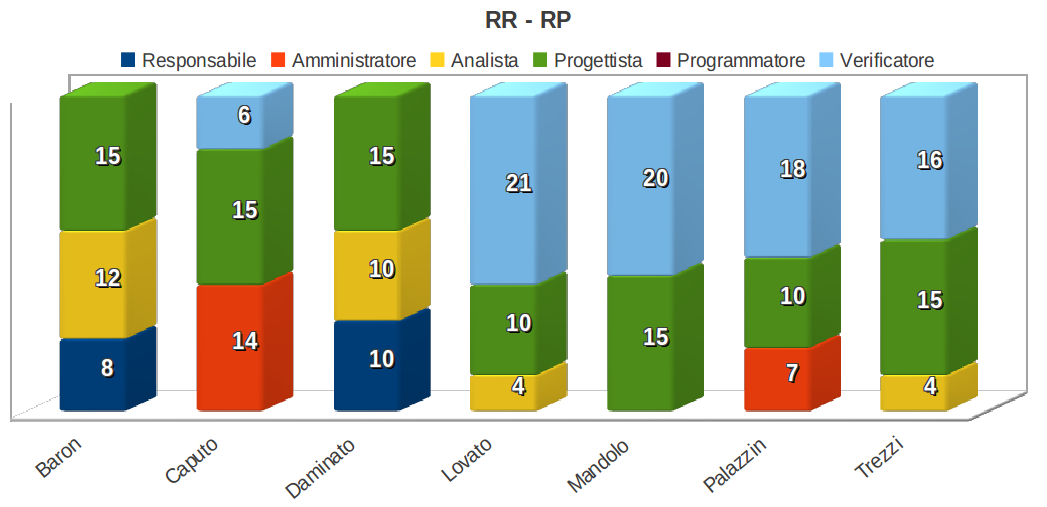
\includegraphics[width=17.2cm, angle=0]{img/PP/RR-RP.png}
\caption{Distribuzione ore RR-RP}
\end{figure}
\newpage

In questo periodo verr\`a suddiviso il lavoro come riportato nella tabella
sottostante:

\begin{table}[h]
\begin{center}
\begin{tabular}{|p{0.17\textwidth}|c|c|c|c|c|}
\hline
& \bo{Resp.}\cellcolor{orange} & \bo{Amm.}\cellcolor{orange} &
\bo{Anl.}\cellcolor{orange} & \bo{Proget.}\cellcolor{orange} &
\bo{Verif.}\cellcolor{orange} \\ \hline

\cellcolor{orange}&&& Lovato(4) & Baron(15) &\\
\bo{Progettazione}\cellcolor{orange}    &  &  &  & Caputo(15)  & \\
\bo{Architetturale}\cellcolor{orange}    &  &  & & Daminato(15)  & \\
\cellcolor{orange}&&&& Mandolo(15) &\\\hline


\bo{Inizio Proget.}\cellcolor{orange}    &  &  & Trezzi(4) & Lovato(10) &
\\ \bo{di Dettaglio 1}\cellcolor{orange}    &  &  & & Palazzin(10) & \\\hline

\bo{Agg. PP (v2)}\cellcolor{orange}    & Baron(5) & Caputo(5) &  & & \\ \hline

\cellcolor{orange}&&&&Trezzi(3)&Lovato(8)\\
\bo{Agg. PQ (v2)}\cellcolor{orange}    &&&&&Mandolo(7) \\
\cellcolor{orange}&&&&&Palazzin(5)\\\hline

\bo{Correzione}\cellcolor{orange}&Daminato&Palazzin(7)&Baron(12)&Trezzi(12)&\\
\bo{docum. RR}\cellcolor{orange}&(10)&&Daminato(10)&&\\\hline

\cellcolor{orange}&&&&&Caputo(6)\\
\cellcolor{orange}&&&&&Lovato(13)\\
\bo{Verifica}\cellcolor{orange}&&&&&Mandolo(13)\\
\cellcolor{orange}&&&&&Palazzin(13)\\
\cellcolor{orange}&&&&&Trezzi(16)\\ \hline

\bo{Controllo e}\cellcolor{orange}&Baron(3)&&&&\\
\bo{Gestione}\cellcolor{orange}&&&&&\\ \hline

\bo{Gestione}\cellcolor{orange}&&Caputo(9)&&&\\
\bo{strumentaz.}\cellcolor{orange}&&&&&\\ \hline

\end{tabular}
\caption{Ripartizione ruoli e attivit\`a RR-RP}
\end{center}
\end{table}

Da subito verranno corretti i documenti della RR che presentano
errori segnalati dal committente. \\
Si pu\`o notare come i vari documenti vengano presi in mano dai ruoli
corretti: AR e SF da Analisti, NP da Amministratore, PP da Responsabile e
Amministratore, PQ da Progettisti nella parte programmatica e Verificatori nella
parte retrospettiva, ST e DP da Progettisti, MU da Programmatori (in veste di
redattori).\\
Nell'attivit\`a di Progettazione Architetturale verr\`a prodotta la
Specifica Tecnica che sar\`a il nostro documento in ingresso alla RP. Verr\`a poi dedicato un p\`o di tempo nel 
cominciare la Progettazione di Dettaglio, in modo da impostare bene il lavoro
che partir\`a a pieno regime subito dopo tale revisione.\\ Parteciperanno per
qualche ora alla progettazione iniziale anche due Analisti, per individuare vincoli ed eventuali rischi tecnologici.\\
\\
Verranno poi portati alla versione 2.0 il Piano di Progetto ed il Piano di
Qualit\`a.\\
\\
Durante l'intero periodo verr\`a inoltre fatta Verifica, Gestione Strumentazione
e Controllo e Gestione delle Attivit\`a.

\newpage


\subsection{RP - RQ}

\vspace{0.5cm}
Periodo compreso tra la RP (07/02/2011) e la RQ (07/03/2011).

\begin{table}[h]
\begin{center}
\begin{tabular}{|l|c|c|c|c|c|c|c|}
\hline
& \bo{Resp.}\cellcolor{orange} & \bo{Amm.}\cellcolor{orange} &
\bo{Anl.}\cellcolor{orange} & \bo{Proget.}\cellcolor{orange} &
\bo{Program.}\cellcolor{orange} & \bo{Verif.}\cellcolor{orange} & \bo{Ore
Totali}\cellcolor{orange} \\ \hline

\bo{Baron}\cellcolor{orange}    &   &    &    & 10 & 10&30 & 50 \\ \hline
\bo{Caputo}\cellcolor{orange}   &   &    &    & 15 & 20&16 & 51 \\ \hline
\bo{Daminato}\cellcolor{orange} &   &   4&    & 15 & 20&12 & 51 \\ \hline
\bo{Lovato}\cellcolor{orange}   &   &   9&    & 15 & 10&17 & 51 \\ \hline
\bo{Mandolo}\cellcolor{orange}  &  5&    &    & 10 & 20&16 & 51 \\ \hline
\bo{Palazzin}\cellcolor{orange} &   &    &    & 20 & 15&15 & 50 \\ \hline
\bo{Trezzi}\cellcolor{orange}   &  8&    &    & 10 & 20&13 & 51 \\  \hline
\bo{TOTALE}\cellcolor{orange} & 13 & 13 & & 95 & 115 & 119 & 355 \\ \hline

\end{tabular}
\caption{Pianificazione oraria RP-RQ}
\end{center}
\end{table}
\vspace{0.5cm}

\bo{Ore totali:} 355.\\

\bo{Costo previsto per il periodo RP-RQ:} \euro\ 6250.

\vspace{0.8cm}
\begin{figure}[htbp]
  \centering
  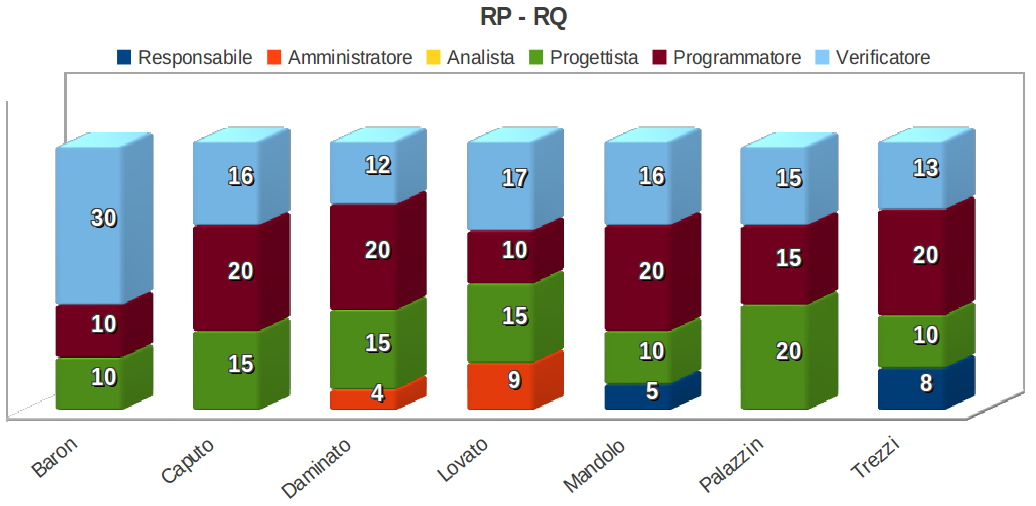
\includegraphics[width=17.2cm, angle=0]{img/PP/RP-RQ.png}
\caption{Distribuzione ore RP-RQ}
\end{figure}
\newpage


In questo periodo verr\`a suddiviso il lavoro come riportato nella tabella
sottostante:

\begin{table}[h!]
\begin{center}
\begin{tabular}{|p{0.17\textwidth}|c|c|c|c|c|}
\hline
& \bo{Resp.}\cellcolor{orange} & \bo{Amm.}\cellcolor{orange} &
\bo{Proget.}\cellcolor{orange} & \bo{Program.}\cellcolor{orange} &
\bo{Verif.}\cellcolor{orange} \\ \hline

\cellcolor{orange}&&&Baron(10) &&\\
\bo{Progettazione}\cellcolor{orange}&&&Daminato(15) &&\\
\bo{di Dettaglio 1}\cellcolor{orange}&&&Lovato(15) &&\\
\cellcolor{orange}&&&Palazzin(5) &&\\
\cellcolor{orange}&&&Trezzi(10)&&\\ \hline

\cellcolor{orange}&&&&Caputo(15) &\\
\cellcolor{orange}&&&&Daminato(15) &\\
\bo{Codifica 1}\cellcolor{orange}&&&&Mandolo(5)&\\
\cellcolor{orange}&&&& Palazzin(10) &\\
\cellcolor{orange}&&&&Trezzi(20)&\\ \hline

\bo{Progettazione}\cellcolor{orange}&&&Caputo(15) &&\\
\bo{di Dettaglio 2}\cellcolor{orange}&&&Mandolo(10) &&\\
\cellcolor{orange}&&&Palazzin(10)&&\\ \hline

\cellcolor{orange}&&&&Baron(5) &\\
\bo{Codifica 2}\cellcolor{orange}&&&&Lovato(10)&\\
\cellcolor{orange}&&&& Mandolo(15)&\\ \hline

\bo{Inizio Test}\cellcolor{orange}&&&&&Baron(15) \\
\bo{di Qualifica}\cellcolor{orange}&&&&&Lovato(17) \\
\cellcolor{orange}&&&&&Trezzi(13)\\ \hline

\bo{Agg. PP (v3)}\cellcolor{orange}  & Trezzi(8) & Daminato(4) &  & & \\ \hline
\bo{Agg. PQ (v3)}\cellcolor{orange}  &  &  &  & &Daminato(6) \\ \hline
\bo{Agg. PQ (v4)}\cellcolor{orange}  &  &  &  & &Caputo(8) \\ \hline

\cellcolor{orange}&&&&Baron(5)&\\
\bo{Manuale}\cellcolor{orange}&&&& Caputo(5) &\\
\bo{Utente (v1)}\cellcolor{orange}&&&&Daminato(5) &\\
\cellcolor{orange}&&&&Palazzin(5)&\\ \hline

\bo{Correzione}\cellcolor{orange}&&&Palazzin(5)&&Mandolo(5)\\
\bo{docum. RP}\cellcolor{orange}&&&&&\\\hline

\cellcolor{orange}&&&&&Baron(15)\\
\cellcolor{orange}&&&&& Caputo(8) \\
\bo{Verifica}\cellcolor{orange}&&&&&Daminato(6) \\
\cellcolor{orange}&&&&&Mandolo(11) \\
\cellcolor{orange}&&&&&Palazzin(15)\\ \hline

\bo{Controllo e}\cellcolor{orange}&Mandolo(5)&&&&\\
\bo{Gestione}\cellcolor{orange}&&&&&\\ \hline

\bo{Gestione}\cellcolor{orange}&&Lovato(9)&&&\\
\bo{strumentaz.}\cellcolor{orange}&&&&&\\ \hline

\end{tabular}
\caption{Ripartizione ruoli e attivit\`a RP-RQ}
\end{center}
\end{table}

Durante la Progettazione di Dettaglio verr\`a stesa la Definizione di
Prodotto.\\
Inizieranno i Test e verr\`a creata una versione preliminare del Manuale Utente.

\newpage


\subsection{RQ - RA}

\vspace{0.5cm}
Periodo compreso tra la RQ (07/03/2011) e la RA (primo appello).

\begin{table}[h]
\begin{center}
\begin{tabular}{|l|c|c|c|c|c|c|c|}
\hline
& \bo{Resp.}\cellcolor{orange} & \bo{Amm.}\cellcolor{orange} &
\bo{Anl.}\cellcolor{orange} & \bo{Proget.}\cellcolor{orange} &
\bo{Program.}\cellcolor{orange} & \bo{Verif.}\cellcolor{orange} & \bo{Ore
Totali}\cellcolor{orange} \\ \hline

\bo{Baron}\cellcolor{orange}    &   &    &    &    & 15& 5 & 20 \\ \hline
\bo{Caputo}\cellcolor{orange}   &  6&    &    &    &  5& 8 & 19 \\ \hline
\bo{Daminato}\cellcolor{orange} &   &    &    &    &   &19 & 19 \\ \hline
\bo{Lovato}\cellcolor{orange}   &   &    &    &  5 & 10& 4 & 19 \\ \hline
\bo{Mandolo}\cellcolor{orange}  &   &    &    &    & 10& 9 & 19 \\ \hline
\bo{Palazzin}\cellcolor{orange} &   &    &    &    &   &20 & 20 \\ \hline
\bo{Trezzi}\cellcolor{orange}   &   &   9&    &    & 10&   & 19 \\  \hline
\bo{TOTALE}\cellcolor{orange} & 6 & 9 & & 5 & 50 & 65 & 135 \\ \hline

\end{tabular}
\caption{Pianificazione oraria RQ-RA}
\end{center}
\end{table}
\vspace{0.5cm}

\bo{Ore totali:} 135.\\

\bo{Costo previsto per il periodo RQ-RA:} \euro\ 2195.

\vspace{0.8cm}
\begin{figure}[htbp]
  \centering
  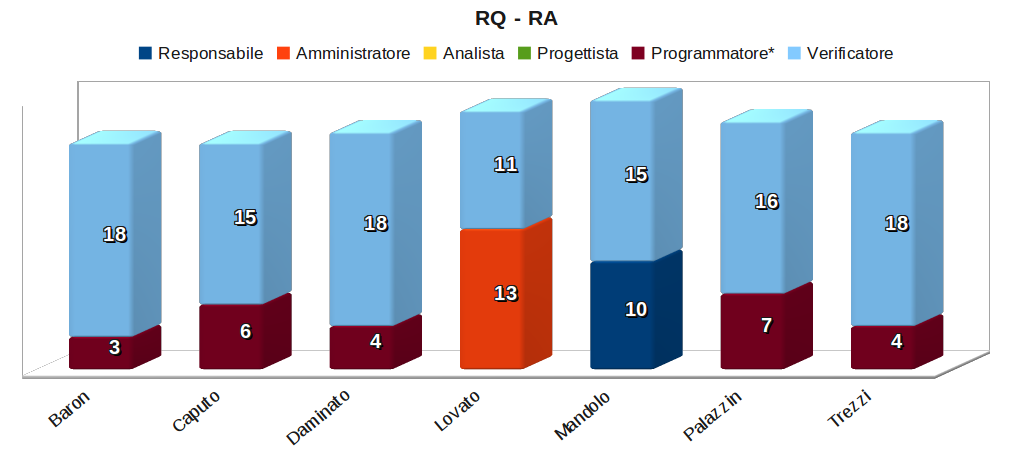
\includegraphics[width=17.2cm, angle=0]{img/PP/RQ-RA.png}
\caption{Distribuzione ore RQ-RA}
\end{figure}
\newpage

In questo periodo verr\`a suddiviso il lavoro come riportato nella tabella
sottostante:

\begin{table}[h!]
\begin{center}
\begin{tabular}{|p{0.17\textwidth}|c|c|c|c|c|}
\hline
& \bo{Resp.}\cellcolor{orange} & \bo{Amm.}\cellcolor{orange} &
\bo{Proget.}\cellcolor{orange} & \bo{Program.}\cellcolor{orange} &
\bo{Verif.}\cellcolor{orange} \\ \hline

\cellcolor{orange}&&&&& Daminato(10)\\
\bo{Test Qualifica}\cellcolor{orange}&&&&& Caputo(8) \\
\cellcolor{orange}&&&&& Palazzin(12)\\ \hline

\bo{Manuale}\cellcolor{orange}&&&& Baron(15)  &\\
\bo{Utente (v2)}\cellcolor{orange}&&&& Lovato(10) &\\
\bo{ITA}\cellcolor{orange}&&&& Trezzi(10) & \\ \hline

\bo{Manuale}\cellcolor{orange}&&&& Caputo(5)&\\
\bo{Utente (v2)}\cellcolor{orange}&&&&  Mandolo(10)&\\
\bo{ENG}\cellcolor{orange}&&&&&\\ \hline

\bo{Agg. PQ (v5)}\cellcolor{orange}  &  &  &  & & Daminato(5) \\
\cellcolor{orange}&&&&&Palazzin(5)\\ \hline

\bo{Correzione}\cellcolor{orange}&&&Palazzin(5)&&Baron(5)\\
\bo{docum. RQ}\cellcolor{orange}&&&&&\\\hline

\cellcolor{orange}&&&&& Daminato(4) \\
\bo{Verifica}\cellcolor{orange}&&&&& Lovato(4) \\
\cellcolor{orange}&&&&& Mandolo(9) \\
\cellcolor{orange}&&&&& Palazzin(3)\\ \hline

\bo{Controllo e}\cellcolor{orange}&Caputo(6)&&&&\\
\bo{Gestione}\cellcolor{orange}&&&&&\\ \hline

\bo{Gestione}\cellcolor{orange}&&Trezzi(9)&&&\\
\bo{strumentaz.}\cellcolor{orange}&&&&&\\ \hline

\end{tabular}
\caption{Ripartizione ruoli e attivit\`a RQ-RA}
\end{center}
\end{table}

Verr\`a inoltre fatta internamente la validazione del sistema per verificare
che vengano soddisfatti tutti i requisiti e che il prodotto realizzato sia
quello atteso.\\
\\
Durante la RA, insieme al committente, verr\`a eseguito il
collaudo formale del prodotto.\\
\\
Dettagli pi\`u specifici di come avverr\`a la qualifica del prodotto sono
presenti nel Piano Di Qualifica.

\newpage


\section{Costi complessivi}

\vspace{0.5cm}
In tutto il periodo di sviluppo del software, verranno complessivamente usate
735 ore per un costo totale di \euro\ 13.460,00.

\vspace{0.3cm}
\begin{table}[h]
\begin{center}
\begin{tabular}{|l|c|c|c|c|c|c|c|}
\hline
& \bo{Resp.}\cellcolor{orange} & \bo{Amm.}\cellcolor{orange} &
\bo{Anl.}\cellcolor{orange} & \bo{Proget.}\cellcolor{orange} &
\bo{Program.}\cellcolor{orange} & \bo{Verif.}\cellcolor{orange} & \bo{Ore
Totali}\cellcolor{orange} \\ \hline

\bo{Baron}\cellcolor{orange}    &  8 &  0 & 12 & 25 & 25 & 35 & 105 \\ \hline
\bo{Caputo}\cellcolor{orange}   &  6 & 14 &  0 & 30 & 25 & 30 & 105 \\ \hline
\bo{Daminato}\cellcolor{orange} & 10 &  4 & 10 & 30 & 20 & 31 & 105 \\ \hline
\bo{Lovato}\cellcolor{orange}   &  0 &  9 &  4 & 30 & 20 & 42 & 105 \\ \hline
\bo{Mandolo}\cellcolor{orange}  &  5 &  0 &  0 & 25 & 30 & 45 & 105 \\ \hline
\bo{Palazzin}\cellcolor{orange} &  0 &  7 &  0 & 30 & 15 & 53 & 105 \\ \hline
\bo{Trezzi}\cellcolor{orange}   &  8 &  9 &  4 & 25 & 30 & 29 & 105 \\ 
\hline

\end{tabular}
\caption{Pianificazione oraria totale}
\end{center}
\end{table}
\vspace{0cm}

Riportiamo qui di seguito un grafico che illustra la ripartizione dei ruoli
sul conto di ore totale.\\

\vspace{0cm}
\begin{figure}[htbp]
  \centering
  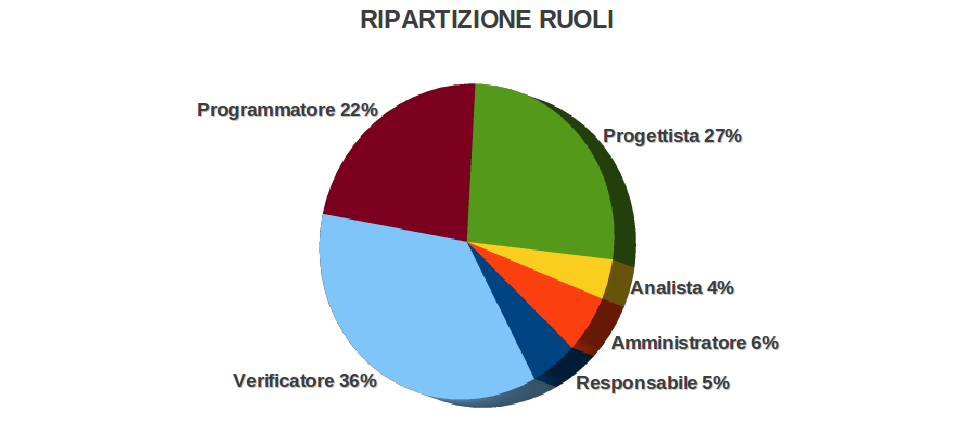
\includegraphics[width=17.2cm, angle=0]{img/PP/RUOLI.png}
\caption{Ripartizione ruoli su ore totali}
\end{figure}

\vspace{0.8cm}
 
Vogliamo fare un piccolo appunto riguardo l'esigua fetta di tempo dedicata
all'analisi. La nostra contabilizzazione economica parte dalla consegna dei documenti per 
la RR (20 Dicembre 2010), momento in cui la parte pi\`u importante dell'analisi \`e stata fatta.
L'analisi che viene riportata in questo grafico fa parte delle
rivisitazioni dei requisiti dopo la RR.\\
\newpage

Questo grafico riporta, in percentuale, il costo dei vari ruoli sul costo totale
del progetto.

\vspace{0cm}
\begin{figure}[htbp]
  \centering
  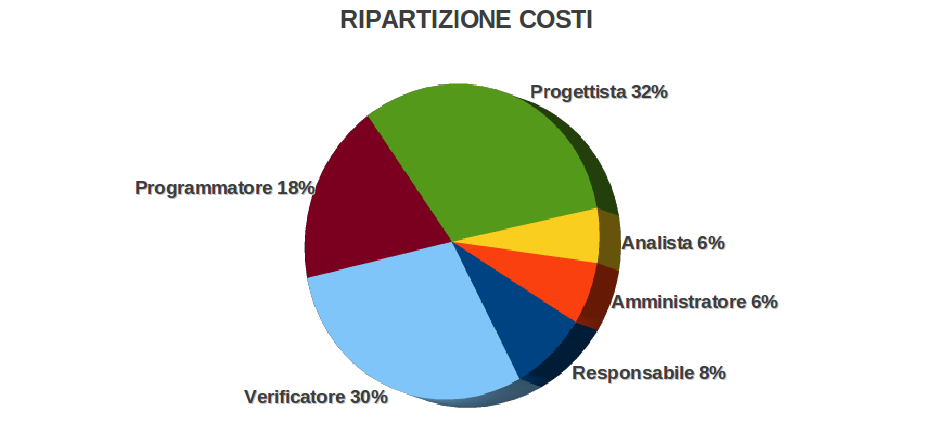
\includegraphics[width=17.2cm, angle=0]{img/PP/COSTI.png}
\caption{Ripartizione costi per ruolo su costo totale}
\end{figure}
\vspace{0.5cm}

Qui di seguito riportiamo la ripartizione oraria per risorsa dei ruoli.

\vspace{0cm}
\begin{figure}[htbp!]
  \centering
  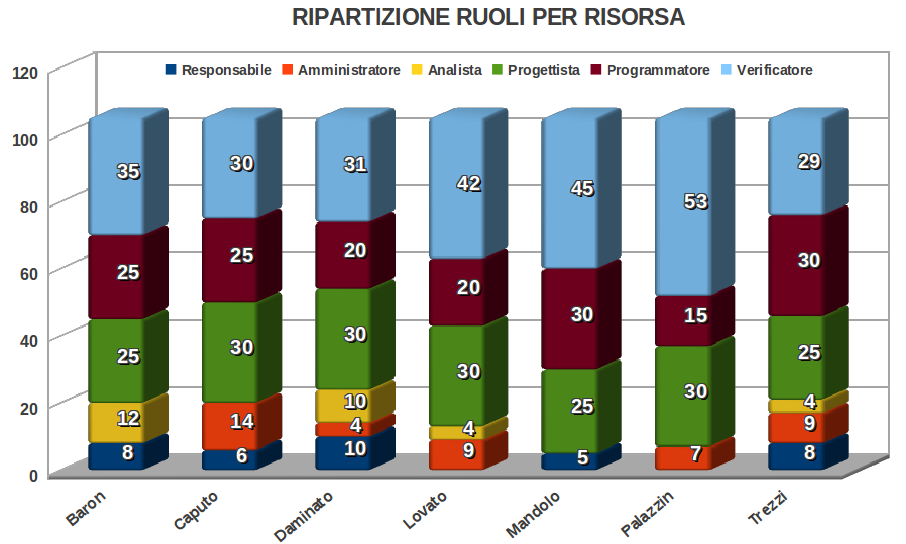
\includegraphics[width=17.2cm, angle=0]{img/PP/RISORSE.png}
\caption{Ripartizione oraria per risorsa dei ruoli}
\end{figure}
\vspace{0.5cm}


\chapter{Consuntivo}

All'interno di questo capitolo sar\`a presentato un confronto con le ore di lavoro
totali spese in ogni fase e le ore di lavoro preventivate. Oltre a questo, il consuntivo 
presenter\`a per ogni fase costi sostenuti e budget rimanente.

\section{Consuntivo in fase RR-RP}

Riportiamo di seguito una tabella con le ore preventivate per ogni attivit\`a
in fase RR-RP e le ore effettivamente utilizzate dagli sviluppatori.

\begin{table}[h]
\begin{center}
\begin{tabular}{|p{0.35\textwidth}|c|c|}
\hline
& \bo{Preventivo}\cellcolor{orange} &
\bo{Consuntivo}\cellcolor{orange}
\\
\hline


\bo{Progettazione Architetturale}\cellcolor{orange} & 64 & 88 \\\hline
\bo{Inizio Proget. di Dettaglio 1}\cellcolor{orange}    & 24 & 13 
\\\hline
\bo{Agg. PP (v2)}\cellcolor{orange}  & 10 & 12\\ \hline
\bo{Agg. PQ (v2)}\cellcolor{orange}  & 23 & 33\\\hline
\bo{Correzione docum. RR}\cellcolor{orange} & 51 & 32\\\hline
\bo{Verifica}\cellcolor{orange}& 61 & 64\\\hline
\bo{Controllo e Gestione}\cellcolor{orange}& 3 & 2 \\\hline
\bo{Gestione strumentaz.}\cellcolor{orange}& 9 & 7\\\hline
\bo{Totale}& 245 & 251\\\hline 
\end{tabular}
\caption{Confronto Preventivo/Consuntivo in fase RR-RP}
\end{center}
\end{table}

Come si pu\`o notare dalla tabella, la progettazione architetturale ad alto
livello ha occupato pi\`u ore di quante preventivate.
La progettazione del sistema era stata sottostimata. 
Conseguentemente le ore di progettazione in dettaglio sono state inferiori
rispetto alle previsioni. 
A compensare le troppe ore impiegate nella progettazione, ci sono state le attivit\`a di correzione
dei documenti dopo gli esiti della RR, che hanno occupato quasi 20 ore in meno del
previsto. Per quanto riguarda le rimanenti attivit\`a, le ore preventivate e le
ore parziali non distano di quantit\`a troppo rilevanti, ad esclusione
dell'aggiornamento del PQ che ha richiesto una decina di ore in pi\`u rispetto al previsto.

\newpage
Riportiamo di seguito un grafico con un confronto tra le ore di lavoro
preventivate, e le ore di lavoro effettive svolte in questa fase.

\vspace{0cm}
\begin{figure}[htbp!]
  \centering
  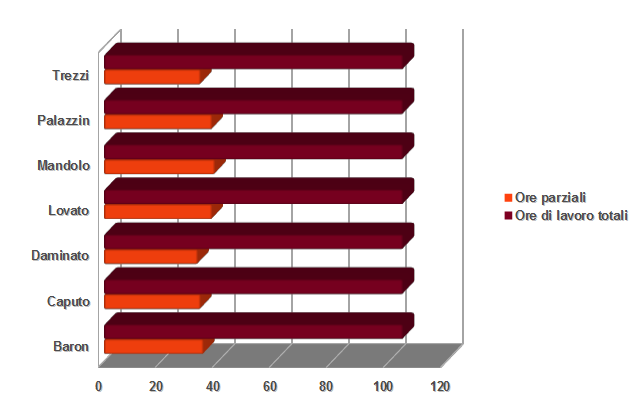
\includegraphics[width=17.2cm, angle=0]{img/PP/ORE-RP.png}
\caption{Rapporto tra ore parziali e ore totali preventivate per membro.}
\end{figure}
\vspace{0.5cm}

Come si pu\`o vedere dal grafico, per ogni membro il monte ore parziale per
questa fase si aggira intorno alle 35 ore, proprio come preventivato, che \`e
circa il 33\% delle ore totali.

\newpage
Riportiamo ora un grafico che mostra le spese sostenute in questa
fase in relazione al budget totale accordato con il committente per lo sviluppo del progetto.

\vspace{0cm}
\begin{figure}[htbp!]
  \centering
  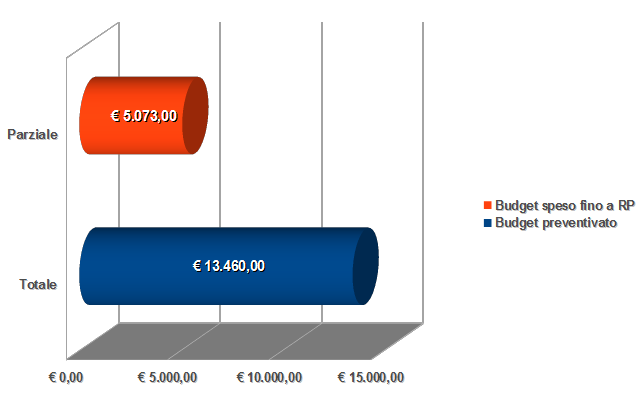
\includegraphics[width=11cm, angle=0]{img/PP/BUDGET-RP.png}
\caption{Stato del budget utilizzato fino a RP}
\end{figure}
\vspace{0.5cm}

Il budget speso \`e stato all'incirca il 37.7\% del budget totale.\\
\\
Inoltre di seguito forniamo anche un grafico a torta a che espone la
ripartizione delle spese per ogni ruolo.

\vspace{0cm}
\begin{figure}[htbp!]
  \centering
  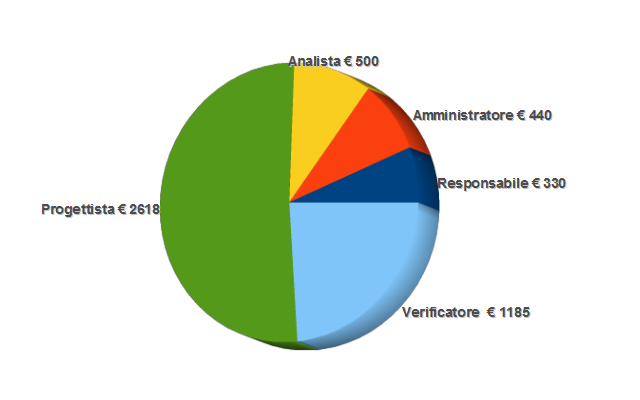
\includegraphics[width=13cm, angle=0]{img/PP/COSTI-RP.png}
\caption{Ripartizione dei costi per ruolo in fase RR-RP}
\end{figure}
\vspace{0.5cm}

In questa fase, la maggior parte delle risorse economiche sono state consumate
dai progettisti e dai verificatori, seguiti dagli analisti che hanno ultimato il
loro lavoro.

\subsection{Rivisitazione Preventivo Fase RP-RQ}

In base al consuntivo ottenuto dalla fase precedente, \`e stato rivisitato il
preventivo per la fase successiva di lavoro, cos\`i da poter riorganizzare le
ore in modo adeguato senza uscire dai limiti orari e di budget impostati nel
preventivo originario.

\begin{table}[h]
\begin{center}
\begin{tabular}{|l|c|c|c|c|c|c|c|}
\hline
& \bo{Resp.}\cellcolor{orange} & \bo{Amm.}\cellcolor{orange} &
\bo{Anl.}\cellcolor{orange} & \bo{Proget.}\cellcolor{orange} &
\bo{Program.}\cellcolor{orange} & \bo{Verif.}\cellcolor{orange} & \bo{Ore
Totali}\cellcolor{orange} \\ \hline

\bo{Baron}\cellcolor{orange}    &   &    &    & 10 & 10 & 30 & 50 \\ \hline
\bo{Caputo}\cellcolor{orange}   &   &    &    & 15 & 20 & 16 & 51 \\ \hline
\bo{Daminato}\cellcolor{orange} &   &   4&    & 15 & 16 & 12 & 51 \\ \hline
\bo{Lovato}\cellcolor{orange}   &   &   9&    & 15 & 10 & 17 & 51 \\ \hline
\bo{Mandolo}\cellcolor{orange}  &  5&    &    & 12 & 16 & 16 & 51 \\ \hline
\bo{Palazzin}\cellcolor{orange} &   &    &    & 20 & 15 & 15 & 50 \\ \hline
\bo{Trezzi}\cellcolor{orange}   &  8&    &    & 15 & 15 & 13 & 51 \\  \hline
\bo{TOTALE}\cellcolor{orange} & 13 & 13 & & 102 & 102 & 119 & 349 \\ \hline

\end{tabular}
\caption{Pianificazione oraria RP-RQ Riorganizzata}
\end{center}
\end{table}
\vspace{0.5cm}

\bo{Ore totali:} 349.\\

Come si pu\`o notare dal grafico le ore sono state ripartite in modo diverso
rispetto al preventivo originario, anche se le differenze sono esigue. Sono
Le ore totali sono ridotte a 349, ossia 6 ore di lavoro in meno, che sono
quelle consumate nella fase precedente. Inoltre le ore di progettazione sono
state aumentate, diretta conseguenza dell'esperienza fatta con la progettazione
nella fase RR-RP. Le ore di codifica sono diminuite, prevedendo che una buona e
dettagliata progettazione richieda meno ore di codifica. Il resto \`e rimasto
invariato.\\
\\Riportiamo di seguito il preventivo in dettaglio delle attivit\`a
riorganizzato.

\begin{table}[h!]
\begin{center}
\begin{tabular}{|p{0.17\textwidth}|c|c|c|c|c|}
\hline
& \bo{Resp.}\cellcolor{orange} & \bo{Amm.}\cellcolor{orange} &
\bo{Proget.}\cellcolor{orange} & \bo{Program.}\cellcolor{orange} &
\bo{Verif.}\cellcolor{orange} \\ \hline

\cellcolor{orange}&&&Baron(10) &&\\
\bo{Progettazione}\cellcolor{orange}&&&Daminato(15) &&\\
\bo{di Dettaglio 1}\cellcolor{orange}&&&Lovato(15) &&\\
\cellcolor{orange}&&&Palazzin(5) &&\\
\cellcolor{orange}&&&Trezzi(15)&&\\ \hline

\cellcolor{orange}&&&&Caputo(15) &\\
\cellcolor{orange}&&&&Daminato(11) &\\
\bo{Codifica 1}\cellcolor{orange}&&&&Mandolo(3)&\\
\cellcolor{orange}&&&& Palazzin(10) &\\
\cellcolor{orange}&&&&Trezzi(15)&\\ \hline

\bo{Progettazione}\cellcolor{orange}&&&Caputo(15) &&\\
\bo{di Dettaglio 2}\cellcolor{orange}&&&Mandolo(12) &&\\
\cellcolor{orange}&&&Palazzin(10)&&\\ \hline

\cellcolor{orange}&&&&Baron(5) &\\
\bo{Codifica 2}\cellcolor{orange}&&&&Lovato(10)&\\
\cellcolor{orange}&&&& Mandolo(13)&\\ \hline

\bo{Inizio Test}\cellcolor{orange}&&&&&Baron(15) \\
\bo{di Qualifica}\cellcolor{orange}&&&&&Lovato(17) \\
\cellcolor{orange}&&&&&Trezzi(13)\\ \hline

\bo{Agg. PP (v3)}\cellcolor{orange}  & Trezzi(8) & Daminato(4) &  & & \\ \hline
\bo{Agg. PQ (v3)}\cellcolor{orange}  &  &  &  & &Daminato(6) \\ \hline
\bo{Agg. PQ (v4)}\cellcolor{orange}  &  &  &  & &Caputo(8) \\ \hline

\cellcolor{orange}&&&&Baron(5)&\\
\bo{Manuale}\cellcolor{orange}&&&& Caputo(5) &\\
\bo{Utente (v1)}\cellcolor{orange}&&&&Daminato(5) &\\
\cellcolor{orange}&&&&Palazzin(5)&\\ \hline

\bo{Correzione}\cellcolor{orange}&&&Palazzin(5)&&Mandolo(5)\\
\bo{docum. RP}\cellcolor{orange}&&&&&\\\hline

\cellcolor{orange}&&&&&Baron(15)\\
\cellcolor{orange}&&&&& Caputo(8) \\
\bo{Verifica}\cellcolor{orange}&&&&&Daminato(6) \\
\cellcolor{orange}&&&&&Mandolo(11) \\
\cellcolor{orange}&&&&&Palazzin(15)\\ \hline

\bo{Controllo e}\cellcolor{orange}&Mandolo(5)&&&&\\
\bo{Gestione}\cellcolor{orange}&&&&&\\ \hline

\bo{Gestione}\cellcolor{orange}&&Lovato(9)&&&\\
\bo{strumentaz.}\cellcolor{orange}&&&&&\\ \hline

\end{tabular}
\caption{Ripartizione ruoli e attivit\`a RP-RQ Riorganizzata}
\end{center}
\end{table}

Anche in questo grafico, si pu\`o notare come siano variate, anche se di poco,
le ore rispettivamente di progettazione fase 1 e fase 2, e di codifica fase 1 e
fase 2. Come gi\`a accennato abbiamo stimato che ad una progettazione pi\`u
dettagliata segua una codifica efficace e meno dispendiosa in termini di
tempistiche.

\newpage
\section{Consuntivo in fase RP-RQ}

Riportiamo di seguito una tabella con le ore preventivate per ogni attivit\`a
in fase RP-RQ e le ore effettivamente utilizzate dagli sviluppatori.

\begin{table}[h]
\begin{center}
\begin{tabular}{|p{0.35\textwidth}|c|c|}
\hline
& \bo{Preventivo}\cellcolor{orange} &
\bo{Consuntivo}\cellcolor{orange}
\\
\hline


\bo{Progettazione di Dettaglio 1}\cellcolor{orange} & 60 & 69 \\\hline
\bo{Progettazione di Dettaglio 2}\cellcolor{orange}    & 36 & 44 
\\\hline
\bo{Codifica 1}\cellcolor{orange}  & 54 & 49\\ \hline
\bo{Codifica 2}\cellcolor{orange}  & 28 & 26\\\hline
\bo{Agg. PP v3.0}\cellcolor{orange} & 12 & 10\\\hline
\bo{Agg. PQ v3.0}\cellcolor{orange}& 6 & 4\\\hline
\bo{Agg. PQ v4.0}\cellcolor{orange}& 8 & 8 \\\hline
\bo{Manuale Utente (v1)}\cellcolor{orange}& 20 & 20\\\hline
\bo{Correzione docum. RP}\cellcolor{orange}& 10 & 9\\\hline
\bo{Verifica}\cellcolor{orange}& 55 & 58\\\hline
\bo{Gestione e Controllo}\cellcolor{orange}& 5 & 4\\\hline
\bo{Gestione Strumentazione}\cellcolor{orange}& 9 & 7\\\hline
\bo{Inizio Test di Qualifica}\cellcolor{orange}& 45 & 39\\\hline
\bo{Totale}& 348 & 347\\\hline 
\end{tabular}
\caption{Confronto Preventivo/Consuntivo in fase RP-RQ}
\end{center}
\end{table}



Come si pu\`o notare dal grafico, le ore preventivate per ogni attivit\`a sono
state rispettate. Notiamo un leggero aumento nelle ore di progettazione, che
come scritto nel preventivo, hanno favorito una progettazione di dettaglio pi�
completa e conseguentemente hanno permesso di occupare meno ore per la codifica.
Vediamo inoltre che le attivit\`a svolte dal responsabile e dagli amministratori
hanno occupato qualche ora in meno rispetto a quanto preventivato, e in totale
tutto ci\`o ha portato ad guadagnare un ora di lavoro sul lavoro totale
previsto.\`E stata anche stilata una versione preliminare del manuale utente.
Insieme ai test di qualifica l'attivit\`a di verifica ha occupato anche in
questa fase una cospicua parte delle ore di lavoro, ossia circa il 28\%.

\newpage
Riportiamo di seguito un grafico con un confronto tra le ore di lavoro
preventivate, e le ore di lavoro effettive svolte in questa fase.

\vspace{0cm}
\begin{figure}[htbp!]
  \centering
  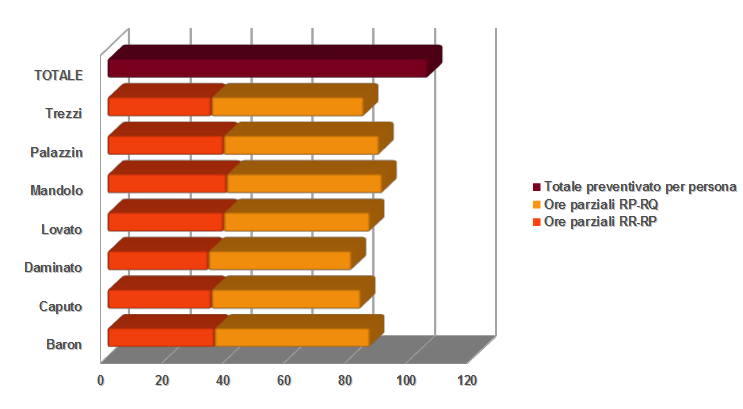
\includegraphics[width=17.2cm, angle=0]{img/PP/ORE-RQ.png}
\caption{Rapporto tra ore parziali e ore totali preventivate per membro.}
\end{figure}
\vspace{0.5cm}


Come stimato, le ore di lavoro svolte in questa fase sono circa 50
ore per ogni componente, che sommate a quelle della precedente fase fanno salire
il monte ore totale a 80 ore circa per persona, pari al 78\% delle ore totali
preventivate. Le ore rimanenti saranno adoperate per il completamento
dell'attivit� non ancora svolte, i test ed il collaudo interno.

\newpage
Riportiamo ora un grafico che mostra le spese sostenute in questa
fase in relazione al budget totale accordato con il committente per lo sviluppo del progetto.

\vspace{0cm}
\begin{figure}[htbp!]
  \centering
  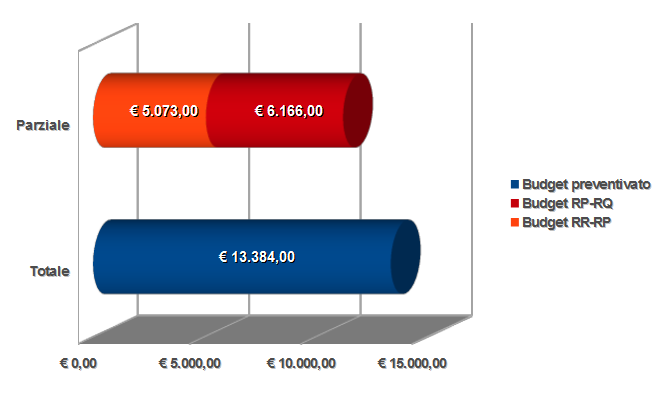
\includegraphics[width=11cm, angle=0]{img/PP/BUDGET-RQ.png}
\caption{Stato del budget utilizzato fino a RQ}
\end{figure}
\vspace{0.5cm}


Il Budget speso in questa fase \`e rimasto molto al di sotto della stima fatta
nel preventivo. Infatti \`e stato consumato il 40\% del budget in questa fase
(5.692 Euro spesi contro 6.250 E preventivati), per un totale di 10.704 Euro di
budget speso finora.


\vspace{0cm}
\begin{figure}[htbp!]
  \centering
  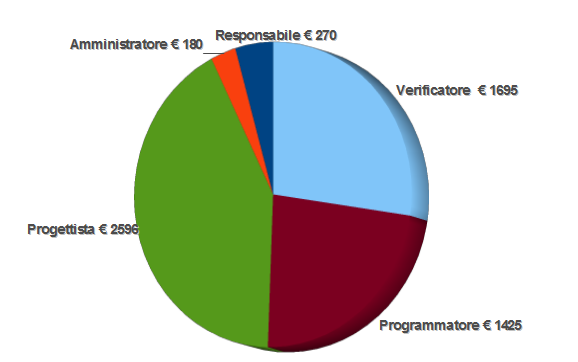
\includegraphics[width=13cm, angle=0]{img/PP/COSTI-RQ.png}
\caption{Ripartizione dei costi per ruolo in fase RP-RQ}
\end{figure}
\vspace{0.5cm}


Come fa chiaramente notare il grafico a torta, anche in questa fase la maggior
parte dei liquidi sono stati consumati dall'attivit\`a svolta dal progettista,
seguiti da programmatori e verificatori.


\chapter{Analisi e gestione dei rischi}
\thispagestyle{fancy}

Questo capitolo ha lo scopo di classificare eventuali problematiche per grado
di pericolosit\`a, di analizzarle e di determinare le azioni da intraprendere per
ridurne i danni. L'attenzione ai rischi sar\`a continua nel corso del
progetto.\\ 
Nonostante il nostro gruppo non abbia ancora una visione completa e dettagliata del 
progetto, i rischi che abbiamo individuato sono riportati nelle seguenti sezioni.

\section{Elenco dei rischi maggiori}

\subsection{Indisposizione dei membri del gruppo}
\bo{Grado di pericolosit\`a}: alto\\
Per i componenti del VT.G questo progetto \`e una delle prime esperienze nel campo della progettazione software in dettaglio. 
La disponibilit\`a dei membri \`e perci\`o uno dei rischi maggiori. 
Assenze causate da problematiche fisiche (malattie, incidenti e imprevisti vari) comporterebbero gravi perdite 
di tempo per tutti gli altri membri e conseguenti ritardi nell'avanzamento del
lavoro.\\
La probabilit\`a di occorrenza di questo rischio direttamente proporzionale alla
frequenza con cui questi incontri si svolgono. 
Si pu\`o affermare che la minor frequenza di riunioni  una conseguenza dell'indisposizione di alcuni membri.
Ad ogni modo la probabilit\`a stimata \`e del 30\%.\\
\\
Ogni componente \`e tenuto a confermare in modo tempestivo la propria presenza
prima di ogni nuovo incontro. I componenti di VT.G risiedono in differenti zone
della regione, i ritrovi devono quindi essere organizzati per tempo e comunicati
a tutti tempestivamente. Ritardi e/o assenza causa trasporti sono difficilmente
gestibili, ma \`e possibile svolgere delle conferenze da casa tramite il
software di videoconferenza Skype.

\subsection{Conoscenza delle Tecnologie Utilizzate}
\bo{Grado di pericolosit\`a}: medio\\
Per la maggior parte dei membri del gruppo questo progetto \`e il primo approccio con tecnologie come GAE, 
perci\`o, almeno inizialmente, questo sistema potrebbe risultare problematico e
creare ritardi nello sviluppo.\\
La probabilit\`a di occorrenza \`e stata stimata del 20\%.\\
\\ 
\`E stato concordato che ogni membro potr\`a seguire un corso proposto
  dall'azienda di un altro capitolato, quindi le basi per l'utilizzo di questo
  sistema saranno assicurate per tutti. Il fattore di rischio perci\`o \`e
  dettato principalmente dalla difficolt\`a del sistema in s\'e. Il linguaggio
  di programmazione adottato (\underline{Java}) non viene considerato come un
  rischio notevole, in quanto studiato durante il corso di laurea in modo
  esauriente. L'unico inconveniente pu\`o essere l'interazione col
  database non relazionale \underline{Google Datastore} che utilizza \underline{GQL}, linguaggio simile a
  \underline{SQL} (trattato sufficientemente nel nostro corso di studio).

\subsection{Usabilit\`a del Prodotto}
\bo{Grado di pericolosit\`a}: basso\\
Il sistema NetMus \`e un buon prodotto di catalogazione e visualizzazione delle
proprie preferenze musicali, ma spesso i lettori Mp3 che di per s\'e sono gi\`a
dispositivi ad alta portabilit\`a mettono a disposizione la visualizzazione del
catalogo multimediale, aggiornato e ordinato. Inoltre sono presenti altri
software simili a NetMus distribuiti sul web come ad esempio LastFM, molto
famoso e utilizzato nella rete. Questo potrebbe ridurre il numero di utenti disposti
ad utilizzare il sistema NetMus.\\
La probabilit\`a di occorrenza del rischio \`e molto variabile, dipendente
sopratutto da come viene svolto il lavoro nelle varie fasi. Ad ogni modo si
stima una probabilit\`a di occorrenza pari al 33\%.\\
\\
Una possibile soluzione \`e quella di decorare il progetto con delle
funzionalit\`a innovative, cos\`\i\ da riuscire ad attirare un maggior numero di clienti.

\subsection{Strumenti d'Utilizzo}
\bo{Grado di pericolosit\`a}: medio\\
Altro fattore di rischio identificato \`e l'utilizzo delle strumentazioni adatte. 
Tutti i membri devono utilizzare le stesse strumentazioni e avere le stesse possibilit\`a nel lavoro. 
Guasti hardware, impossibilit\`a di connettersi alla rete \underline{Internet},
mancanza di strumentazioni software adatte comportano ritardi, incompatibilit\`a e sopratutto confusione. \\
La probabilit\`a di occorrenza \`e del 40\%.\\
\\
Ogni membro del gruppo, 
rispettando quanto scritto nel documento
\emph{NormeDiProgetto-\versionenormeprogetto.pdf}, si \`e procurato la
strumentazione software adatta prima dell'inizio del lavoro. In caso di problemi
pi\`u complessi ogni membro \`e invitato a comunicare il fatto
all'amministratore che cercher\`a una soluzione idonea.

\subsection{Informazioni Aggiuntive sui Brani Musicali}
\bo{Grado di pericolosit\`a}: medio\\
I file Mp3 da cui si reperiscono i brani spesso non possiedono informazioni
complete, anzi una buona parte di questi file non contiene affatto informazioni, perci\`o la libreria virtuale 
di un utente risulterebbe composta da molti brani senza titolo, autore e altre
informazioni essenziali.\\
La probabilit\`a di occorrenza \`e del 60\%.\\
\\
Per rendere la libreria virtuale completa di tutte le informazioni si \`e ben pensato di implementare una 
funzione di ricerca automatica nel server dai record di tutti i brani registrati, cos\`\i\ da completare 
quelli incompleti. Nei casi estremi inoltre sar\`a resa possibile una funzione
di inserimento delle informazioni manualmente.

\section{Strategie di gestione dei rischi}

Di seguito riportiamo un elenco delle strategie per la gestione dei rischi sopra
elencati.\\

Le strategie adoperate sono:
\begin{itemize}
	\item Evitare il rischio, ossia cercare di adeguarlo in modo da eliminare la
	condizione rischiosa. 
	\item Mitigare il rischio, riducendone le probabilit\`a o le conseguenze.
	\item Accettare il rischio, in maniera attiva (attuando comunque un piano
	contingente) o passiva (intervenendo solo nel momento in cui il rischio si
	manifester\`a).
\end{itemize}

Ognuna di queste strategie  stata adottata per trovare una soluzione
ad ogni specifico rischio in modo che arrecasse meno danno possibile allo
sviluppo del progetto.\\

\section{Rischi incontrati nelle fasi di sviluppo}

\subsection{Rischi nella fase RR - RP}
Il rischio maggiore che il gruppo ha dovuto affrontare in questa fase \`e stato il
dover correggere e rivedere alcuni documenti per intero. Ci\`o non ha gravato
sul monte ore totali, infatti come si pu\`o vedere da questo Piano Di Progetto era gi\`a
stato previsto un ritorno sui documenti dopo l'ingresso in Revisione dei
Requisiti. Perci\`o il rischio non \`e stato rilevato.\\
\\
Il grado di pericolosit\`a del rischio esposto al paragrafo 6.1.2 si \`e
ridotto. Ci\`o \`e dettato dal fatto che i membri hanno potuto avere una prima
esperienza personale con i tutorial di GoogleAppEngine e con un corso tenuto su quest'ultimo dal 
personale della Miriade SPA. La probabilit\`a di occorrenza del rischio \`e comunque alta.\\
\\
Il gruppo \`e riuscito a mitigare in questa fase la probabilit\`a di occorrenza del
rischio esposto al paragrafo 6.1.1. Si \`e
infatti deciso di svolgere la maggior parte del lavoro da casa, con comunicazioni effettuate via Skype ogni qualvolta fosse
stato necessario. Gli incontri ufficiali sono stati quindi ridotti al minimo,
con la conseguenza di aver ottenuto una partecipazione attiva e completa di
tutti i membri.\\
\\

\subsection{Rischi nella fase RP - RQ}
In questa fase, uno dei rischi maggiori che ha dovuto affrontare il gruppo \`e
stato il dover riorganizzare il preventivo di questa stessa fase. \`E stato
necessario rivisitare il preventivo poich\`e nella fase precedente erano state
utilizzate pi\`u ore di quelle previste, ed era necessario rientrare nei
limiti proposti nel preventivo iniziale. Questo rischio \`e stato affrontato attivamente, 
il gruppo infatti ha investito nelle ore di progettazione svolgendo un lavoro
pi\`u dettagliato che ha conseguentemente portato ad un lavoro di codifica meno
complesso del previsto, permettendo quindi di guadagnare alcune ore di lavoro e
di rientrare nel preventivo.\\
\\
La condizione rischiosa del fattore alla sezione 6.1.2 \`e stata quasi
completamente annullata, grazie allo studio continuo e
all'esperienza ottenuta lavorando su GAE e GWT.\\
\\
Il fattore rischioso alla sezione 6.1.5 si \`e abbassato notevolmente, dato che
nello sviluppo del progetto abbiamo implementato la possibilit\`a di aggiungere
o modificare le informazioni riguardanti un brano. Quindi ora ogni brano mp3 con
informazioni parzialmente o del tutto mancanti potr\`a comunque essere
completato nei suoi campi direttamente dall'utente. \`E comunque ancora un
rischio ``attivo'' dato che il completamento delle informazioni, qualora il
programma non riuscisse a reperire le informazioni dal database centrale, resta
un compito che pu\`o svolgere solamente l'utente.
\listoftables
\addcontentsline{toc}{chapter}{Indice Tabelle}
\listoffigures
\addcontentsline{toc}{chapter}{Indice Figure}
\end{document}
